\documentclass[border=3mm]{standalone}

\usepackage{tikz}
\usetikzlibrary{decorations.markings,arrows.meta}

\begin{document}
	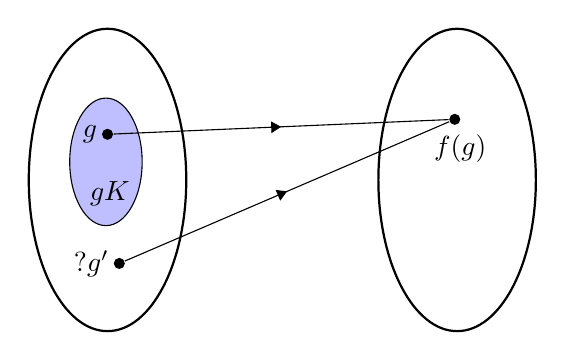
\begin{tikzpicture}
		\draw[thick]  (-1.93,-0.52) ellipse (1 and 1.92);
		\draw[thick]  (2.51,-0.52) ellipse (1 and 1.92);
		\draw[fill=blue!25]  (-1.95,-0.29) ellipse (0.46 and 0.81);
		\node[circle,fill=black,inner sep=0pt,minimum size=4pt,label={left,xshift=2pt:$g$}] (1) at (-1.93,0.06) {};
		\node[circle,fill=black,inner sep=0pt,minimum size=4pt,label={below,xshift=2pt:$f(g)$}] (2) at (2.48,0.25) {};
		\node[circle,fill=black,inner sep=0pt,minimum size=4pt,label={ left,xshift=2pt:$?g'$}] (3) at (-1.78,-1.58) {};
		\node at (-1.9,-0.7) {$gK$};
	\begin{scope}[decoration={
		markings,
		mark=at position 0.5 with {\arrow{Triangle}}
	}]
		\draw[postaction={decorate}] (1) -- (2);
		\draw[postaction={decorate}] (3) -- (2);
	\end{scope}
	\end{tikzpicture}
\end{document}